\chapter{Energy Approximators} 
\label{chapter-4} 

\begin{itemize}
\item As we will sse in next chapter, EMMA uses a measure of outlyingness, ideally true energy
\item However difficult to train, explore two simple alternative measures: ... those are approximations
\item Obtained training a DAE (see section below) explains the model and then next section explain where approximations come from.
\item Finally, we conclude with experiment to choose the best
\end{itemize}

%----------------------------------------------------------------------------------------
%	SECTION 
%----------------------------------------------------------------------------------------

\section{Autoencoder}

Principle AE. unsupervised training. MSE, x, r(x), recon, encoder, decoder. Why useful to do input. Let us distinguish two cases: under/overcomplete

%-----------------------------------
%	SUBSECTION 
%-----------------------------------
\subsection{Undercomplete}
\begin{itemize}
\item undercomplete, hidden representation, forces to keep only useful information, latent space...
\item explain diagrams. when we minimize MSE, we minimize norm of vector r-x
\end{itemize}

\begin{figure}[!h]
\centering
\begin{subfigure}{.5\textwidth}
  \centering
  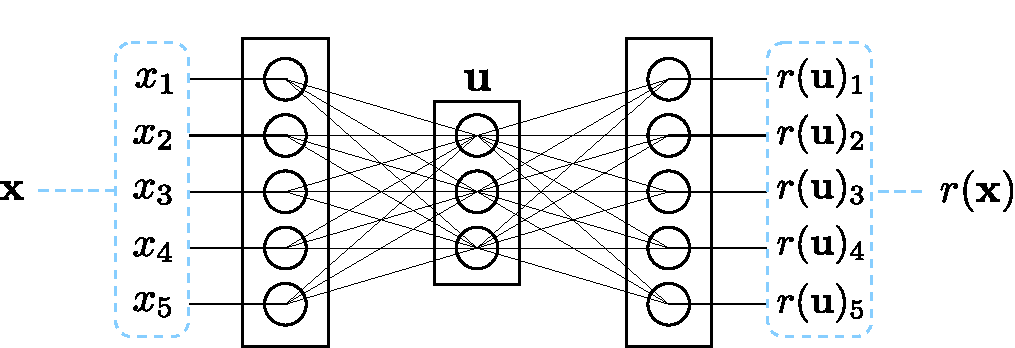
\includegraphics[width=.75\linewidth]{figures/autoencoder-undercomplete}
  \caption{Autoencoder}
  \label{fig:ae}
\end{subfigure}%
\begin{subfigure}{.5\textwidth}
  \centering
  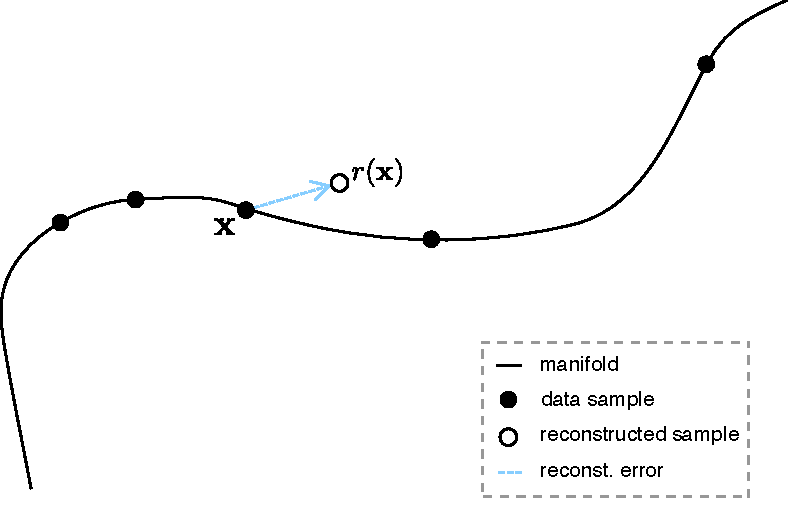
\includegraphics[width=.75\linewidth]{figures/reconstruction}
  \caption{Data space}
  \label{fig:ae-process}
\end{subfigure}
\caption{Reconstruction}
\label{fig:test}
\end{figure}

%-----------------------------------
%	SUBSECTION 
%-----------------------------------
\subsection{Overcomplete}

overcomplete to avoid copying - corruption becomes denoising. Can be used for denoising of signals. explain diagrams

\begin{figure}[!h]
\centering
\begin{subfigure}{.5\textwidth}
  \centering
  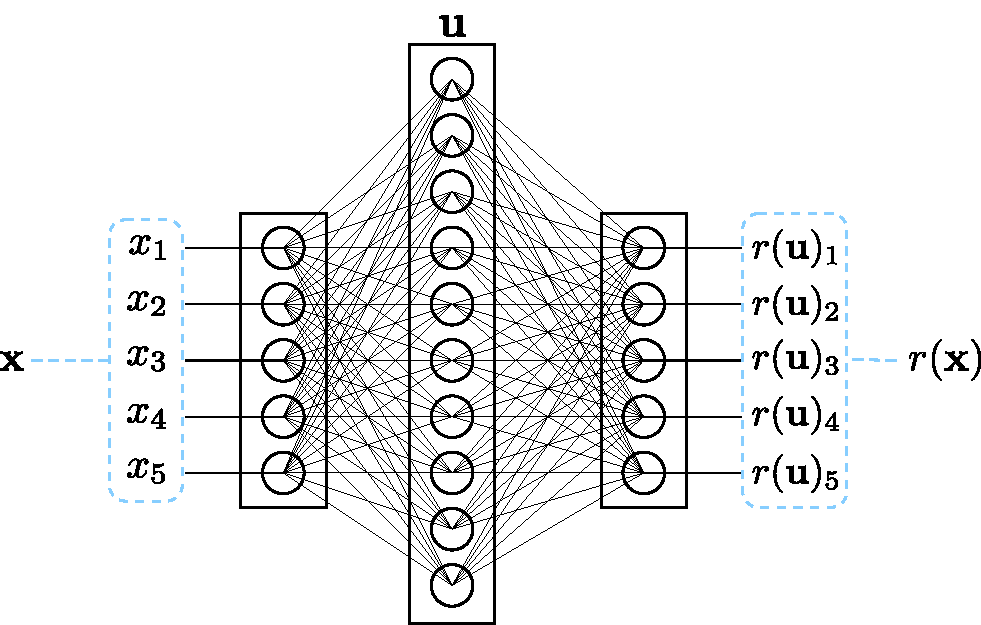
\includegraphics[width=.75\linewidth]{figures/autoencoder-overcomplete}
  \caption{Denoising Autoencoder}
  \label{fig:dae}
\end{subfigure}%
\begin{subfigure}{.5\textwidth}
  \centering
  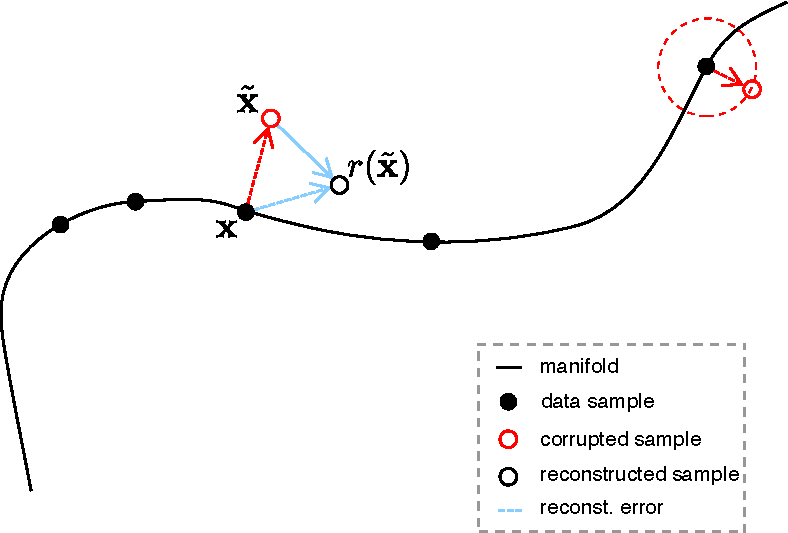
\includegraphics[width=.75\linewidth]{figures/reconstruction-denoising}
  \caption{Data space}
  \label{fig:dae-process}
\end{subfigure}
\caption{Reconstruction with corruption}
\end{figure}

%----------------------------------------------------------------------------------------
%	SECTION 
%----------------------------------------------------------------------------------------

\section{Reconstruction norm \& Potential}

Small introduction. Explain article of Bengio intuitively and how it leads to score is reconstruction. 
$$ r(\tilde{\textbf{m}}_i) - \textbf{m}_i \propto \frac{\partial \log p(\textbf{m}_i)}{\partial \textbf{m}_i} $$ 
Explain how this relates to vector field. Show circle and vector field. \\
Then show idea of other paper intuitively. Potential. Conditions. Force.
$$\Psi_i = -\int (r(\tilde{\textbf{m}}_i) - \textbf{m}_i)d\textbf{m}_i$$
Develop not show, just mention it is proofed in paper and not difficult.
$$ \Psi_i = -\int f(\textbf{m}_i)d\textbf{m}_i - \frac{1}{2} \lVert \textbf{m}_i + \textbf{b}_r \rVert_2^2 + \text{const} $$
in this work sigmoid is only activation used but other can be easliy used (see paper).
$$ \Psi_i =  -\sum_k \log(1 + \text{exp}(W_{.k}^T \textbf{m}_i + b_k^h)) + \frac{1}{2} \lVert \textbf{m}_i - \textbf{b}_r \rVert_2^2 + \text{const}$$


%----------------------------------------------------------------------------------------
%	SECTION 
%----------------------------------------------------------------------------------------

\section{Experiment I}

We expect potential be better, because better grounded. 
Describe generation manifolds + parametric functions. Train AE with noise. experimental setup in appendix. Evaluate on grid. Two manifolds formulas. Mention manifold and their particular form were not chosen for a particular reason.
\begin{figure}[!h]
\centering
\begin{subfigure}{.5\textwidth}
  \centering
  
\includegraphics[width=.4\linewidth]{figures/logo-uliege}
  \caption{Wave manifold}
  \label{fig:wave-manifold-only}
\end{subfigure}%
\begin{subfigure}{.5\textwidth}
  \centering
  
\includegraphics[width=.4\linewidth]{figures/logo-uliege}
  \caption{Circle manifold}
  \label{fig:circle-manifold-only}
\end{subfigure}
\caption{Two manifolds}
\end{figure}

Show results+ observatiions (explain why there are sources, explain why less convergence in center of wave (because more accumulation)) + conclusion we will use potential (better results, more robuts, more theoretically grounded). Table of six figures.

%----------------------------------------------------------------------------------------
%	SECTION 
%----------------------------------------------------------------------------------------

\section{Limitations}

Explain easy but not easily extensible to images/sounds. Mention alternatives. Our goal is not to analyze best energy approximator bt to show that roughly any approx can be used to solve our problem.
\href{https://arxiv.org/pdf/1606.03439.pdf}{alternative}